% latex_demo.tex 

\documentclass{article}
\usepackage{graphicx} % for figures
\usepackage{float}
\usepackage[export]{adjustbox}
\begin{document}

\title{Homework Work 3 - Physics 240}
\author{Tin Tran}

\maketitle

\section{Introduction}

This is an exercise to test the approximation of $e^x$ using the Taylor expansion in the form of: \newline

\begin{equation}\label{eqn:epi}e^x = 1 + x + \frac{x^2}{2!} + \frac{x^3}{3!} + ... = \lim_{N \to \infty} S(x,N)
\end{equation} \newline
Where S(x,N) is the partial sum. The figure below shows the plots of the absolute fractional error $|S(x,N)-e^x|/e^x$ versus N. As we can see, this method is not good for approximating $e^x$ when x $<$ 0 because there will be a discontinuation in the graph, using this model, the series will have alternating + and -, and that result in round of error.

% you have to run/typeset latex twice to get references to take effect

\begin{figure}[H]
\centering{
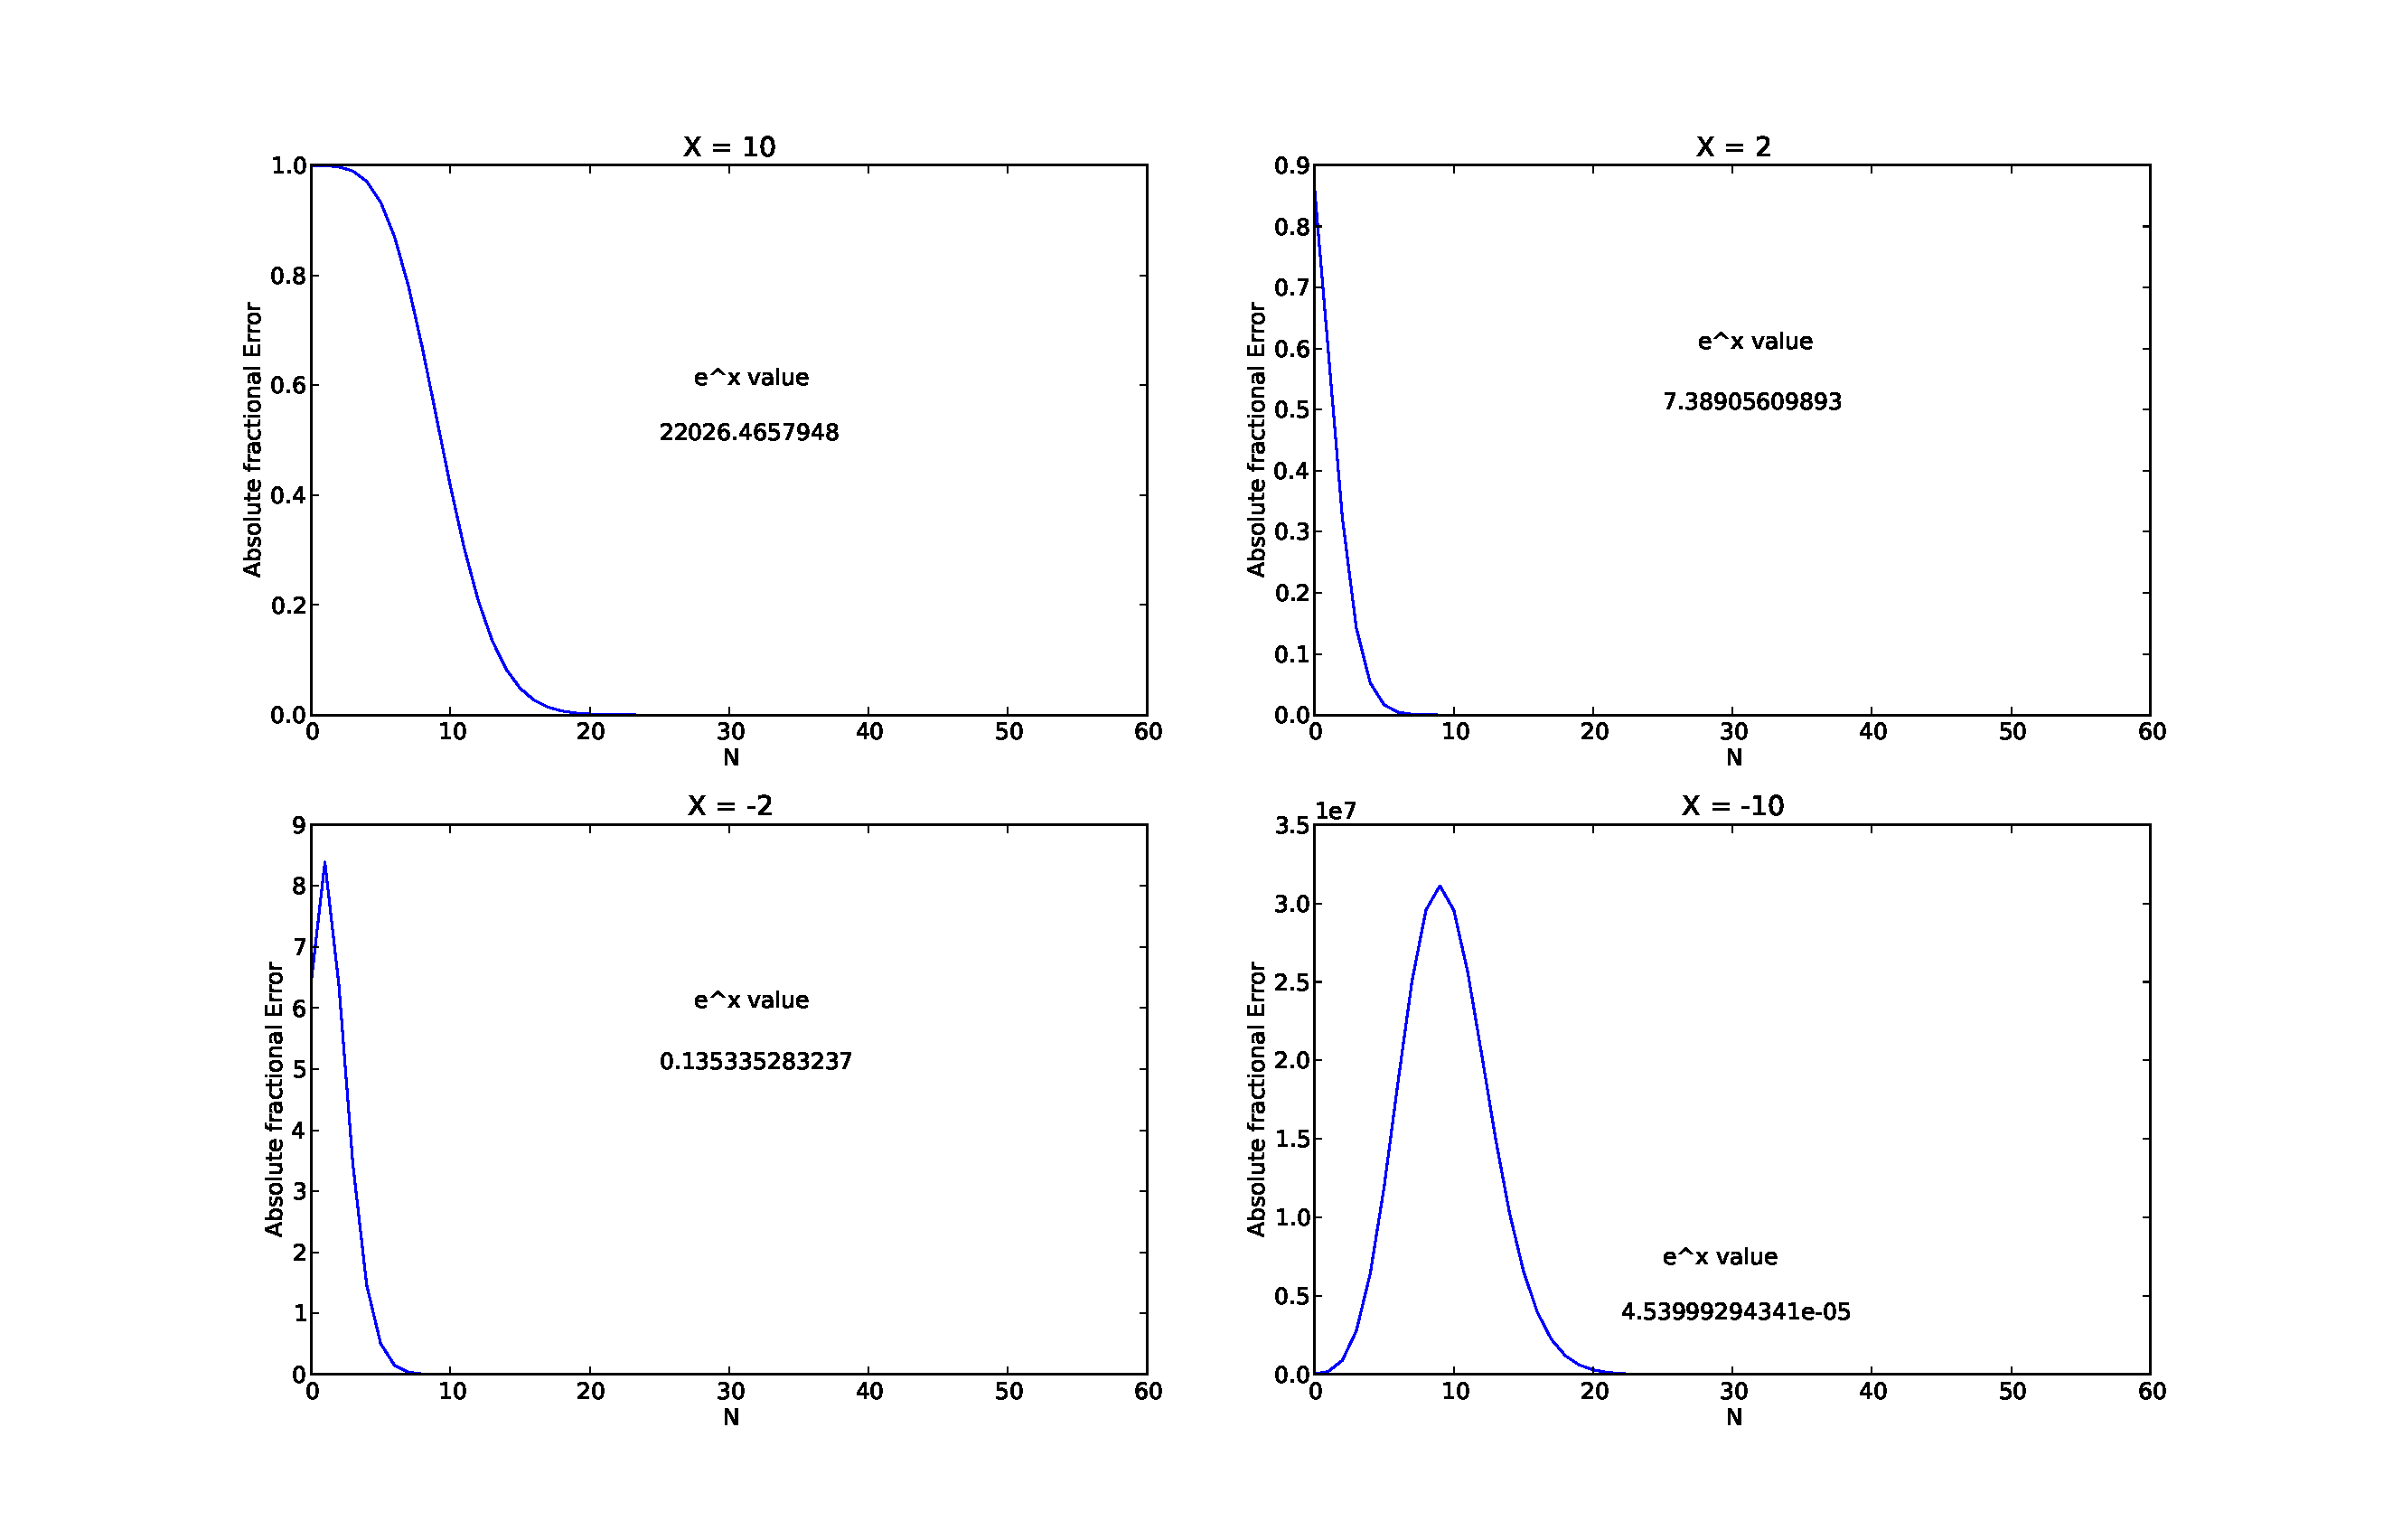
\includegraphics[max size={\textwidth}{\textheight}]{original.eps}
\caption{Approximation using the formula in (1) for $e^x$}
}
\end{figure}

\section{Modified model}

Using the new identity $e^x = 1/e^{-x} = 1/S(-x,N)$, there are less round of error because there is no negative, so there's nothing to substract. This results in a smoother curve for the fractional error versus N, as shown in the figure below
\begin{figure}[H]
\centering{
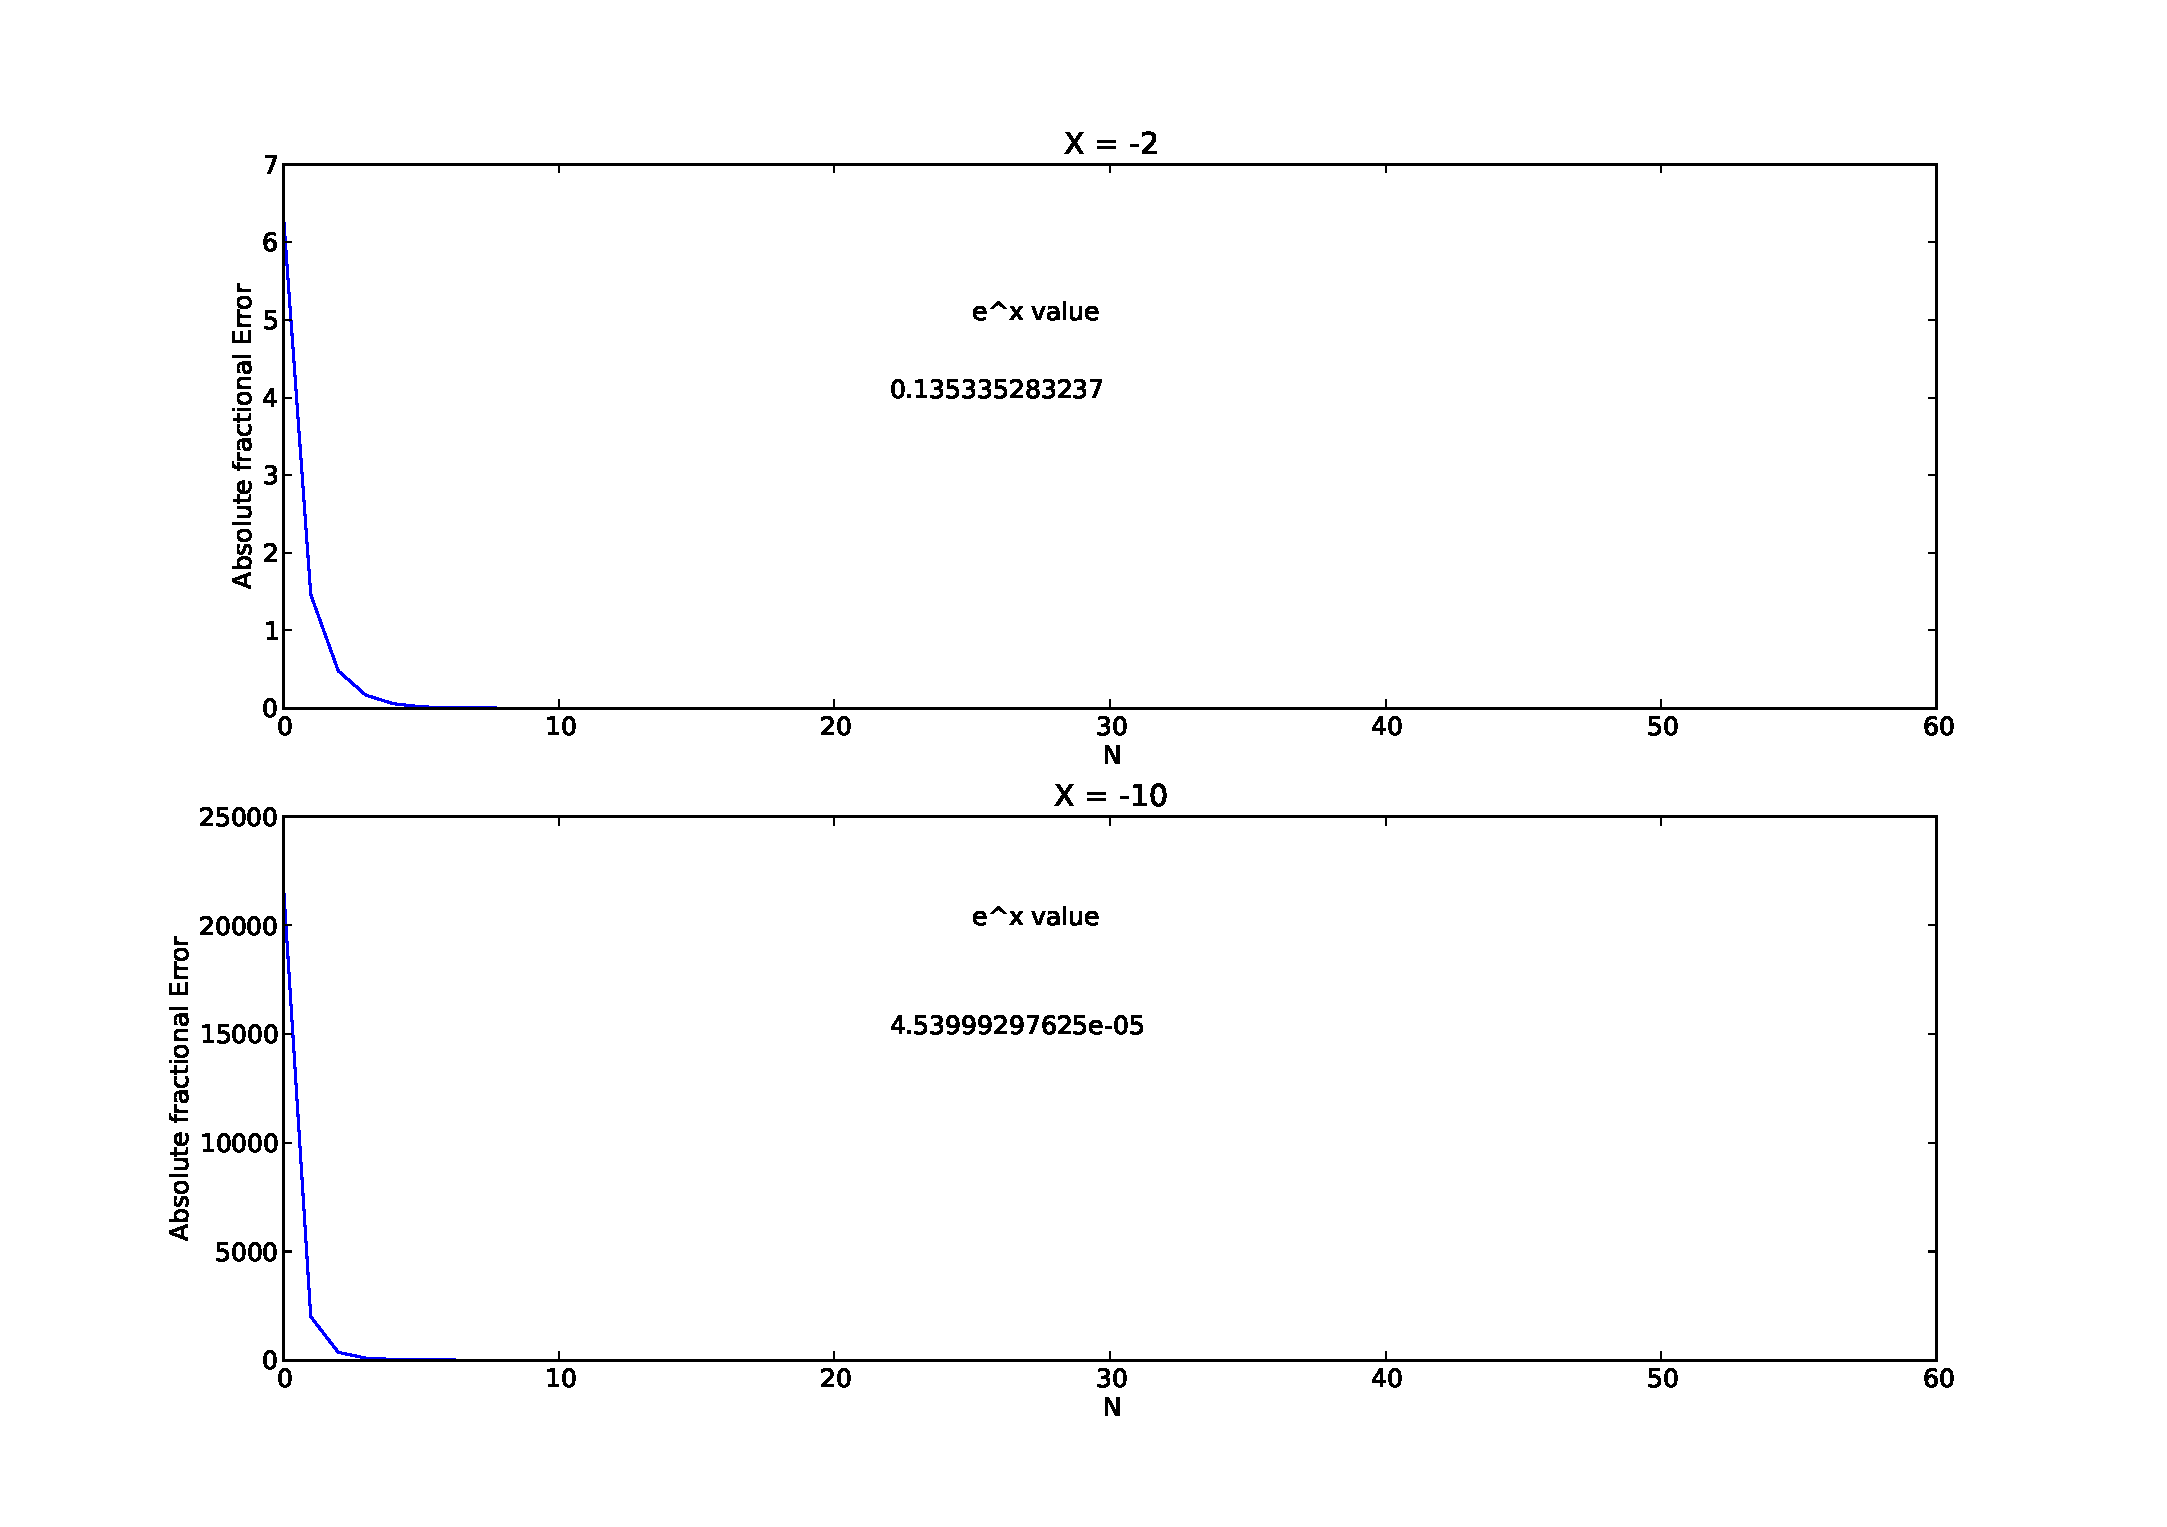
\includegraphics[max size={\textwidth}{\textheight}]{modified.eps}
\caption{Approximation using the new identity for $e^x$}
}
\end{figure}

\end{document}